%% Generated from main.tex by scripts/revision/jnsm_compile.py.
%% Manuscript source for the Journal of Network and Systems Management (Springer Nature).
%% Converted from the Elsevier CAS template on 16 September 2026; the previous source is kept at
%% v2_soc_alert_prioritization/docs/revision/wp9/superseded/2026-09-16_pre_jnsm_main_cas.tex.
\documentclass[pdflatex,sn-basic,Numbered]{sn-jnl}

\usepackage{graphicx}
\usepackage{amsmath,amssymb}
\usepackage{booktabs}
\usepackage{array}
\usepackage{enumitem}
\usepackage{url}
\usepackage{orcidlink}


% generated by scripts/revision/wp8_build_manuscript_assets.py
\newcommand{\NAlerts}{2,655,821}
\newcommand{\NCriticalAlerts}{9,204}
\newcommand{\NCriticalIntervals}{32}
\newcommand{\NCandidates}{157}
\newcommand{\NTuned}{145}
\newcommand{\NUnseenAlerts}{113}
\newcommand{\StaticClassCovered}{8}
\newcommand{\StaticClassFPMedian}{18}
\newcommand{\StaticSOneKeyCovered}{21}
\newcommand{\StaticSZeroKeyCovered}{21}
\newcommand{\StaticRSevKeyCovered}{18}
\newcommand{\StaticKeyFPMedian}{77}
\newcommand{\TieBlockMax}{430,178}
\newcommand{\TieExpectedFPMedian}{0.6}
\newcommand{\TieOrderShareMin}{99}
\newcommand{\TieCutoffMembersMinP}{85}
\newcommand{\TieCutoffMembersMaxP}{97}
\newcommand{\TieCutoffMembersMedianP}{96.5}
\newcommand{\TieCutoffMembersMinClass}{37}
\newcommand{\DeferredCritical}{9,047}
\newcommand{\DeferredShare}{98.3}
\newcommand{\DeferredMappingRejected}{8,999}
\newcommand{\DeferredPrecisionRejected}{8,996}
\newcommand{\DeferredShareSeverity}{20.7}
\newcommand{\SZeroReversalShare}{98.6}
\newcommand{\PrimaryMinP}{0.75}
\newcommand{\ReplayInvestigations}{11,508}
\newcommand{\ReplayClassCovered}{13}
\newcommand{\ReplayClassFP}{9,285}
\newcommand{\ReplayClassStarvedShare}{99.4}
\newcommand{\ReplaySOneKeyCovered}{30}
\newcommand{\ReplaySOneKeyFP}{11,013}
\newcommand{\ReplaySOneKeyStarvedShare}{97.2}
\newcommand{\ReplaySZeroKeyCovered}{28}
\newcommand{\ReplaySZeroKeyFP}{9,345}
\newcommand{\ReplaySZeroKeyStarvedShare}{98.1}
\newcommand{\ReplayRSevKeyCovered}{25}
\newcommand{\ReplayRSevKeyFP}{9,308}
\newcommand{\ReplayRSevKeyStarvedShare}{98.8}
\newcommand{\ReplaySevOnlyCovered}{8}
\newcommand{\ReplaySevOnlyFP}{11,479}
\newcommand{\ReplaySevOnlyStarvedShare}{99.7}
\newcommand{\ReplayFIFOCovered}{0}
\newcommand{\ReplayFIFOFP}{11,508}
\newcommand{\ReplayFIFOStarvedShare}{100.0}
\newcommand{\ReplaySixtyShare}{2.1}
\newcommand{\ReplaySixtyShareMax}{12.3}
\newcommand{\PeakBacklogMin}{44,399}
\newcommand{\PeakBacklogMax}{632,519}
\newcommand{\HoldoutSOneKeyGroups}{9, 20, 8, 8, 8}
\newcommand{\ForwardSOneKey}{13}
\newcommand{\ForwardP}{5}
\newcommand{\UWFRows}{95,871}
\newcommand{\UWFAttackRows}{47,965}
\newcommand{\UWFCredentialShare}{90.68}
\newcommand{\UWFSpearman}{0.872}
\newcommand{\UWFMADWeighted}{1.88}
\newcommand{\UWFMADUnweighted}{0.70}
\newcommand{\UWFJaccardEightFive}{0.50}
\newcommand{\UWFSharedConnections}{326}
\newcommand{\RevisionLateSOneKey}{23}
\newcommand{\RevisionBeforeSOneKey}{7}
\newcommand{\key}{\textsubscript{key}}
\newcommand{\Rsev}{R\textsubscript{sev,key}}

\begin{document}

\title[Evaluating security alert prioritization under limited capacity]{Evaluating Security Alert Prioritization under Limited Capacity: Rule Granularity, Score Ties, and Coverage Tradeoffs}

\author*{\fnm{Murat} \sur{Moran}\,\orcidlink{0000-0001-5557-4827}}\email{murat.moran@giresun.edu.tr}

\affil*{\orgdiv{Department of Computer Engineering}, \orgname{Giresun University}, \orgaddress{\city{Giresun}, \postcode{28200}, \country{T\"{u}rkiye}}}

\abstract{Security operations centers must prioritize alerts under limited investigation capacity, but ranking improvements can conceal tradeoffs between attack-step coverage, false-positive burden, and critical-alert retrieval. We examine these tradeoffs on the AIT Alert Dataset: eight scenarios and \NAlerts{} alerts. A matched-information protocol compares \NCandidates{} candidates using nested selection, static rankings, and chronological single-analyst replay. With class-level rule information, subnormal Gaussian fuzzy number scores and simpler formulas covered the same number of critical intervals in every scenario. Primary tests provided no evidence of a difference in false-positive burden at the first 100 positions. Identifier-level rule precision increased static critical-interval coverage from \StaticClassCovered{} to \StaticSOneKeyCovered{} of \NCriticalIntervals{} intervals, while formulas differed in false-positive burden and replay outcomes. Large tied blocks supplied \TieCutoffMembersMinP--\TieCutoffMembersMaxP{} of the first 100 positions for the probability-proxy score, making tie order consequential. At 12 investigations per hour, the highest-coverage ranker reached \ReplaySOneKeyCovered{} intervals but left \ReplaySOneKeyStarvedShare\% of critical alerts uninvestigated; \RevisionLateSOneKey{} covered intervals were first investigated at or after their end. Identifier hold-out produced heterogeneous coverage of 8--20 intervals, with uneven critical-alert support across groups. Exploratory policy and service-unit analyses retain the class-level coverage equality but show that stricter mapping purity can remove identifier-level gains and that grouping changes the coverage--retrieval gap. On AIT, rule history, score ties, and investigation capacity changed the tradeoffs between interval coverage, false-positive burden, and critical-alert retrieval. Interval coverage remains a temporal proxy, not confirmed attack detection.}

\keywords{Security operations center, Alert management, Alert prioritization, Evaluation methodology, Ranking ties, Queue replay}

\maketitle

% =====================================================================================
\section{Introduction}
\label{sec:introduction}

Security operations centers (SOCs) receive far more alerts than analysts can inspect, and most alerts are benign or low-impact~\citep{Axelsson2000BaseRate,Alahmadi2022FalsePositives,Yang2024SOCAlerts,Tariq2025AlertFatigue}. Alert prioritization therefore has to answer a management question: given limited investigation capacity, which alerts should be examined first~\citep{Jalalvand2025AlertPrioritisation}? Which alerts analysts see depends on the ranking score, the tie-breaking rule, and investigation capacity. These management choices affect prioritization alongside detection quality. A queue can be evaluated by its false-positive burden, retrieval of high-severity alerts, coverage of distinct attack steps, and investigation timing. A score that improves one of these objectives can leave the others unchanged or worse.

\paragraph{Motivation for a matched comparison.}
An earlier preprint introduced the SGFN alert representation and scalar score~\citep{Moran2026RiskAversePreprint}. An audit of an unpublished comparison motivated the common inputs, isolated fitting, and separate interval- and alert-level outcomes used here. Online Resource~1, Section~S2 documents the version history and audit scope.

We compare existing scores, including SGFN, using matched inputs. The experiments examine how historical rule information and tied scores affect rankings. They also measure tradeoffs between interval coverage, investigation burden, and critical-alert retrieval.

\paragraph{Research questions.}
\begin{enumerate}[label=RQ\arabic*,leftmargin=*]
\item Given identical inputs and an identical selection rule, does class-level SGFN improve critical-step interval coverage or false-positive burden relative to simpler scores? Coarse inputs create large score cells: formulas prioritizing the same cells may yield identical coverage even when their numerical scores differ.
\item What do historical rule precision, score granularity, and tie ordering contribute to static rankings, and why are critical alerts deferred?
\item Do static differences survive chronological arrival and limited investigation capacity?
\item How far do the observed coverage gains generalize to detector identifiers that were absent from fitting, and to future scenarios?
\end{enumerate}

\paragraph{Contributions.}
\begin{itemize}[leftmargin=*]
\item A matched-information evaluation that separates changes in historical rule granularity from changes in scoring formula. Nine class-level formula scores have identical static interval coverage, whereas learned models and identifier-level formulas have distinct outcomes (Sections~\ref{sec:static} and~\ref{subsec:drivers}).
\item A quantitative diagnosis of score ties and critical-alert deferral under the declared mapping and severity policy. Tie order strongly affects false-positive burden, and rejected low-precision rules account for most deferred critical alerts (Sections~\ref{subsec:ties} and~\ref{subsec:deferral}).
\item Evidence that interval coverage, timely investigation, and alert-level retrieval diverge under overload, together with support-aware identifier hold-out diagnostics and a forward-scenario replay (Sections~\ref{sec:replay} and~\ref{sec:generalization}).
\item A reproducible protocol with \NCandidates{} candidates, nested selection, declared tie ordering, fitting-isolation checks, and separately identified exploratory extensions (Section~\ref{sec:protocol}).
\end{itemize}

Online Resource~1, Section~S2 separates what the preprint, the earlier version, and this paper contribute; the archive supplies the protocol and verification records (see Statements and Declarations).

% =====================================================================================
\section{Related work}
\label{sec:related}

\paragraph{SOC alert triage.} Operational studies and surveys document the burden of false or benign alerts and alert fatigue~\citep{Alahmadi2022FalsePositives,Yang2024SOCAlerts,Tariq2025AlertFatigue,Jalalvand2025AlertPrioritisation}. Other approaches cluster or correlate alerts, use provenance or ATT\&CK context, or learn context-aware policies~\citep{Julisch2003AlarmClustering,Hassan2019NoDoze,Garcia2025ROSCA,Wang2024AlertPro,vanEde2022DeepCASE}. They use information beyond per-alert severity and rule statistics, so their results are not direct comparators here. Our comparison is deliberately limited to scores computable from the same per-alert inputs.

\paragraph{Alarm management in network and systems management.} Alarm correlation and fault localization address large alarm streams~\citep{Jakobson1993AlarmCorrelation,Steinder2004FaultLocalization}, while inconsistent alarm definitions complicate comparisons~\citep{Wallin2009AlarmDefinition}. Security triage adds an explicit investigation budget~\citep{Tong2020MovingHaystack}. Our replay uses that budgeted framing as an evaluation device: capacity is declared, arrival is causal, and the queue discipline is measured rather than proposed.

\paragraph{Prior evaluation designs.} Relevant studies combine parts of this design (Table~\ref{tab:designs}). AIT's published rate score ranks detectors for filtering~\citep{Landauer2024AITADS}. CATS evaluates modular risk scores and transfer~\citep{Uetz2026CATS}, while TEQ uses temporal splits and simulated queue prioritization~\citep{Gelman2023TEQ}. DeepCASE studies chronological semi-automatic operation~\citep{vanEde2022DeepCASE,Teuwen2025RulesetTuning}. Day-forward chaining has also been used for alert prioritization~\citep{Aminanto2020DayForward}. CSOC models relate uninvestigated alerts to staffing and scheduling~\citep{Ganesan2017OperationalEffectiveness} and quantify throughput, quality, and cost tradeoffs~\citep{Shah2019Tradeoffs}. Budgeted investigation, human-feedback deferral, and dynamic prioritization provide further operational precedents~\citep{Tong2020MovingHaystack,Jalalvand2025L2DHF,KimDan2025Dynamic}. These components are established; here we examine their combined effects on ranking comparisons with matched inputs.

We examine how information granularity and queue ordering change the interpretation of score comparisons, using matched-input ranking experiments, chronological service replay, and identifier exclusion on AIT. A score can cover many intervals while relying heavily on historical identifiers and tie ordering. Its first investigations may occur after those intervals end, and most critical records may remain uninvestigated. We do not claim a new scoring method, a first queue evaluation, or superiority over the contextual and adaptive systems reviewed above.

\begin{tableorg}[t]
\centering
\caption{Closest prior evaluation designs, compared on what they rank, the information they use, how they split data, and how they evaluate operation. Entries describe designs; performance numbers are not comparable across these data sets.}
\label{tab:designs}
\footnotesize
\setlength{\tabcolsep}{3pt}
\begin{tabular}{>{\raggedright\arraybackslash}p{0.15\textwidth}>{\raggedright\arraybackslash}p{0.10\textwidth}>{\raggedright\arraybackslash}p{0.22\textwidth}>{\raggedright\arraybackslash}p{0.22\textwidth}>{\raggedright\arraybackslash}p{0.20\textwidth}}
\toprule
Study & Ranked object & Information & Splitting & Operational evaluation \\
\midrule
AIT data set~\citep{Landauer2024AITADS} & Detectors & Alert rates in attack phases and a normal window & Scores aggregated over all eight scenarios & Detector filtering; no queue model \\
CATS~\citep{Uetz2026CATS} (preprint) & Alerts & Modular risk hypotheses, parameter alternatives & Transfer across eight alert data sets & Threshold-free metrics; no service model \\
TEQ~\citep{Gelman2023TEQ} (preprint) & Incidents & Learned model over incident features & Time-ordered months; decay with and without retraining & Queue times reassigned to reordered incidents \\
DeepCASE case study~\citep{Teuwen2025RulesetTuning} & Event sequences & Rule tuning and label balance & Case study on one deployment & Classification and explanation quality \\
Budgeted policies~\citep{Tong2020MovingHaystack} & Alert types & Costs, budgets, adversary model & Simulated adversary & Defender loss under budgets \\
DeepCASE~\citep{vanEde2022DeepCASE} & Event sequences & Context sequences, operator cluster decisions & Chronological & Workload and risk measures \\
L2DHF~\citep{Jalalvand2025L2DHF} (preprint) & Alerts & Adaptive deferral, simulated human feedback & Online learning in a simulated SOC & Analyst time, processed/unprocessed alerts \\
\midrule
This paper & Alerts & Severity, uncertainty, class- or identifier-level rule reliability & Leave-one-scenario-out, identifier hold-out, forward chaining & Static top-$k$ and single-analyst service replay \\
\bottomrule
\end{tabular}
\end{tableorg}

\paragraph{Evaluation pitfalls.} Base rates, closed-world assumptions, and data-set labels limit headline detection metrics~\citep{Axelsson2000BaseRate,SommerPaxson2010ClosedWorld,Ring2019NIDSDatasets}. NDCG summarizes graded relevance but does not distinguish many alerts from one step from coverage of many steps~\citep{Jarvelin2002NDCG}. Tie-breaking bias is an established evaluation problem: secondary ordering can affect apparent system quality~\citep{Cabanac2010TieBias}. Tied scores make rank metrics depend on within-block order; our diagnostics use the tied-order expectation of \citet{McSherryNajork2008TiedScores}. With interval labels, calibrated probabilities concern an interval-labelled positive, not maliciousness~\citep{ZadroznyElkan2002Calibration,NiculescuMizilCaruana2005Calibration,Guo2017Calibration}.

\paragraph{Fuzzy and severity-based scoring.} Fuzzy sets~\citep{Zadeh1965FuzzySets} underlie fuzzy rule-based intrusion detection~\citep{Tsang2007FuzzyIDS}, and fuzzy-number ranking methods order uncertain quantities~\citep{Chen1985FuzzyRanking}. Severity policies can be keyed to ATT\&CK tactics~\citep{MITREAttack} or to vulnerability scores such as CVSS~\citep{FIRSTCVSS40}, whose relation to exploitation risk is contested~\citep{Allodi2014CVSSExploits,Jacobs2020ExploitPrediction}. Here severity values come from an author-defined policy and are treated as assumptions. Alert aggregation addresses a different but related design choice: the unit presented for investigation~\citep{Landauer2022Aggregation}. Our grouped replay varies that unit without claiming to reproduce a learned aggregation system.

% =====================================================================================
\section{Matched-information comparison protocol}
\label{sec:protocol}

The original 157-candidate comparison protocol and its six primary tests were frozen before those runs. Exploratory identifier-support diagnostics, interval-end timing, and forward replay follow a 26 October 2026 amendment written before computing those additional outcomes. A separate 30 October 2026 amendment specifies tie-policy, mapping-policy, severity, target-alignment, and grouped-service sensitivity analyses after the original results were known; these are exploratory extensions. These extensions do not change the original selection rule or primary testing family. Specifications and verification records identify the code and inputs used.

\subsection{Data, labels, and triage targets}

The AIT Alert Dataset~\citep{AITAlertDataset2023,Landauer2024AITADS} contains alerts from Wazuh, Suricata, and AMiner for eight multi-step attack scenarios in simulated enterprise networks~\citep{Landauer2023MaintainableLogs}. All \NAlerts{} alerts are ranked; none is sampled (Table~\ref{tab:data}). Attack phases are given as time intervals. An alert is an \emph{interval-labelled positive} if its timestamp lies in a half-open attack interval $[s,e)$; this label does not establish that the alert itself is malicious. Each phase receives a severity from an author-defined policy; phases with severity at least $\tau=8$ define 32 \emph{critical-step intervals}, four per scenario, all containing alerts, and \NCriticalAlerts{} critical alerts.

\begin{tableorg}[t]
\centering
\caption{Held-out scenarios. Mapped: share of alerts whose native identifier is mapped to an attack phase by the outer training scenarios (label-free for the held-out scenario). Unseen-identifier alerts: alerts whose (detector, native key) never occurs in the training scenarios.}
\label{tab:data}
\resizebox{\textwidth}{!}{\begin{tabular}{lrrrrrr}
\toprule
Scenario & Alerts & Critical alerts & Critical intervals & Horizon (h) & Mapped (\%) & Unseen-identifier alerts \\
\midrule
fox & 473,104 & 408 & 4 & 119.9 & 88.8 & 0 \\
harrison & 593,948 & 3,385 & 4 & 120.0 & 71.6 & 0 \\
russellmitchell & 45,544 & 743 & 4 & 95.7 & 25.3 & 0 \\
santos & 130,779 & 908 & 4 & 95.9 & 8.7 & 99 \\
shaw & 70,782 & 165 & 4 & 143.5 & 8.9 & 2 \\
wardbeck & 91,257 & 85 & 4 & 120.0 & 7.1 & 6 \\
wheeler & 616,161 & 554 & 4 & 119.9 & 70.0 & 0 \\
wilson & 634,246 & 2,956 & 4 & 143.8 & 68.6 & 6 \\
\midrule
Total & 2,655,821 & 9,204 & 32 & 958.7 & -- & 113 \\
\bottomrule
\end{tabular}
}
\end{tableorg}

We report three outcomes and never merge them:
\begin{itemize}[leftmargin=*]
\item \emph{critical-step interval coverage@k}: the fraction of critical intervals containing at least one of the first $k$ alerts (primary, $k=100$). We show covered counts because coverage changes in steps of one interval out of four per scenario;
\item \emph{FP@k}: interval-labelled negatives among the first $k$ alerts (primary, jointly with coverage);
\item \emph{alert-level critical recall} and deep-queue effort, and in replay the numbers of critical alerts investigated and uninvestigated at the horizon.
\end{itemize}
A covered interval means that an alert inside its time window was ranked or investigated; it is a temporal coverage proxy, not confirmed discovery of the attack step.

\subsection{Common inputs}
\label{subsec:inputs}

All class-level and identifier-level scores are computed from the following per-alert inputs; the operational references use one of them, the timestamp, or a native detector field. The dataset contains 93 native identifiers: rules, signatures, or component keys. Mapping an identifier to an attack phase requires support of at least 5, at least 3 positives, interval precision of at least 0.5, and phase purity of at least 0.7. Identifiers that fail these requirements in the fitting scenarios remain unknown. Severity $c$ is the mapped phase severity, with a default of 5 for unknown identifiers. Uncertainty $u \in [0, 0.5]$ is a per-phase table value. Class reliability $h$ estimates the interval-positive frequency in each (detector, mapped class) cell. We shrink it toward the detector prior with $\lambda=50$ and clip it to $[0.05, 0.95]$. Identifier-level reliability $\hat h_{\mathrm{key}}$ is the same shrunk frequency per native key. Reliability is \emph{cross-fitted}. Each training scenario $j$ is classified using a mapping fitted without $j$, so its labels cannot determine its own mapping. Held-out labels are excluded from fitting. The native detector references rank by Wazuh \texttt{rule.level} (larger first) and Suricata signature severity (smaller first) separately. Missing native values remain missing and sort after available values, with timestamp/hash ordering among missing records; they are not imputed across detector scales.

For a fitted cell with $n$ records and $a$ interval-labelled positives, and detector prior $p_d=a_d/n_d$, the estimator is
\begin{equation}
 h=\operatorname{clip}_{[0.05,0.95]}\!\left(\frac{a+50p_d}{n+50}\right).
\end{equation}
The same expression defines $\hat h_{\mathrm{key}}$ using native-key counts. An absent cell or key falls back to the clipped detector prior, then the clipped global prior if that detector has no fitting records; fitting fails if neither prior is available. The severity and uncertainty values in Table~\ref{tab:policy} are assumptions fixed for the primary analysis. Mapping precision is the positive fraction of a key's records, and phase purity is the largest phase-specific positive count divided by the number of records positive in any attack interval.

\begin{table}[t]
\centering
\caption{Author-defined primary input policy. Critical intervals have severity at least 8. The unknown row applies to identifiers rejected by the training-only phase mapping.}
\label{tab:policy}
\small
\begin{tabular}{lrr}
\toprule
Phase & Severity $c$ & Uncertainty $u$ \\
\midrule
network scans & 2 & 0.10 \\
service scans & 2.5 & 0.10 \\
dirb & 3 & 0.20 \\
wpscan & 3 & 0.20 \\
webshell & 8.5 & 0.35 \\
cracking & 6.5 & 0.20 \\
reverse shell & 9 & 0.35 \\
privilege escalation & 9.5 & 0.35 \\
service stop & 7.5 & 0.20 \\
dnsteal & 9 & 0.35 \\
data exfiltration & 9 & 0.35 \\
unknown & 5 & 0.50 \\
\bottomrule
\end{tabular}
\unskip
\end{table}

\subsection{Comparison families and selection}

Table~\ref{tab:families} lists the 13 families. The SGFN family combines the inputs heuristically. S0 is the historical score $c + \kappa u c \ln h$ with $\kappa=1$, which can reverse severity order. S1 uses the same form, restricting $\kappa$ so that $1 + \kappa u \ln h > 0$ on the declared domain. S2 is $c\,h^{\kappa u}$. Identifier-level variants replace $h$ by $\hat h_{\mathrm{key}}$.

\begin{table}[t]
\caption{Comparison families (\NCandidates{} candidates; \NTuned{} tuned in every inner fold). Scores use the inputs of Section~\ref{subsec:inputs}; operational references use a single input, the timestamp, or a native detector field.}
\label{tab:families}
\small
\setlength{\tabcolsep}{4pt}
\begin{tabular}{>{\raggedright\arraybackslash}p{0.17\textwidth}>{\raggedright\arraybackslash}p{0.38\textwidth}>{\raggedright\arraybackslash}p{0.33\textwidth}}
\toprule
Family & Score & Grid \\
\midrule
Operational references & oldest first (FIFO), newest first (LIFO), native rule level, native Suricata severity, $c$ (O\textsubscript{sev}), $h$ (O\textsubscript{rel}) & untuned \\
H & $0.7c + 3h$ (historical weighted) & untuned \\
W & $\alpha c/10 + (1-\alpha) h$ & $\alpha \in \{0, 0.1, \dots, 1\}$ \\
A & $a\,c/10 + b\,h - d\,u/0.5$, $a+b+d=1$ & simplex, step 0.1 (66) \\
M & $c\,h^{a} e^{-bu}$ & $a \in \{0,0.25,0.5,1,2,4\}$, $b \in \{0,1,2,4,8\}$ \\
P & $h\,c$ (probability proxy) & untuned \\
C & $h c - (1-h) C_{FP}$ & $C_{FP} \in \{0,1,2.5,5,10\}$ \\
L1 & logistic regression for $y$ on $(c,u,h)$, score $\hat p\,c$ & $C \in \{0.01, 1, 100\}$ \\
L2 & gradient-boosted regressor on relevance & max depth $\in \{2,3\}$ \\
R & $\hat h_{\mathrm{key}}$ and $c\,\hat h_{\mathrm{key}}$ (\Rsev) & untuned \\
S0, S0\key & $c + \kappa u c \ln h$ ($\hat h_{\mathrm{key}}$), $\kappa = 1$ & untuned \\
S1, S1\key & $c(1 + \kappa u \ln h)$, domain-constrained & $\kappa \in \{0,0.1,\dots,0.6,0.6676\}$ \\
S2, S2\key & $c\,h^{\kappa u}$ (heuristic) & $\kappa \in \{0,0.5,1,2,4,8\}$ \\
\bottomrule
\end{tabular}
\end{table}

Evaluation is leave-one-scenario-out. Within the seven training scenarios, every tuned candidate is scored in leave-one-training-scenario-out inner folds, with all fitting repeated inside each inner fold. The selection rule maximizes macro coverage@100, then minimizes macro FP@100, then maximizes NDCG@100, then prefers the simplest candidate; it applies to every tuned family (Figure~\ref{fig:protocol}). NDCG is a selection tie-breaker, not a primary endpoint. L2 predicts $r_i/10=y_i s_i^*/10$, where $y_i$ denotes membership in any attack interval and $s_i^*$ is the maximum severity of those intervals; this is interval-derived relevance, not a maliciousness label. The NDCG definition, learner configurations, and fallback rules are in Online Resource~1, Section~S1. All preprocessing is repeated within the fitting boundary.

\begin{figure}[t]
\centering
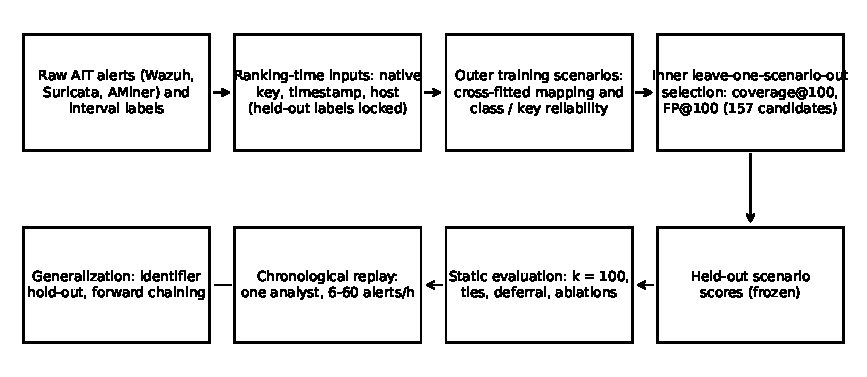
\includegraphics[width=\textwidth]{generated/figures/fig_protocol.pdf}
\caption{Data flow. Held-out labels are locked while inputs are fitted and candidates selected; scores are then frozen for static evaluation and replay.}
\label{fig:protocol}
\end{figure}

\subsection{Ordering, replay, and statistics}

Alerts are ordered by score (descending), then timestamp (ascending), then a SHA-256 hash of the alert identifier. We report tie diagnostics beside the primary results. For linear metrics such as FP@100, we compute exact expectations under uniform ordering within tied blocks, following \citet{McSherryNajork2008TiedScores}. For coverage, which is nonlinear in the ranking, we use 100 seeded within-block permutations.

The replay admits alerts at their timestamps into a backlog. One analyst investigates one alert at a time, non-preemptively, with equal service time at 12 alerts per hour (primary) and 6, 30, and 60 per hour (sensitivity); these rates are assumptions. Each replay runs from the scenario's first alert to its last, with no initial backlog or draining. At equal timestamps, arrivals enter before selection. The analyst selects the best-ranked alert already in the backlog. LOSO replay is arrival-causal conditional on an offline-fitted ranker, whose training scenarios can be later in calendar time than the test scenario. An investigation is counted at its start, including a start whose service completion falls beyond the horizon. It covers an interval only if the investigated alert's own timestamp lies in it. Coverage can therefore be credited after the interval ends; we separately count first investigations before the exclusive interval end and at or after it. These timings do not establish attack detection.

Scenarios are the units of analysis ($n=8$). The prespecified family compares S1 with A, M, and P on coverage@100 and FP@100, giving six tests. Each two-sided paired sign-flip test enumerates all $2^8$ sign patterns, with Holm adjustment across the family~\citep{Holm1979Sequential}. The smallest attainable raw $p$ is $2/256$. Exactness refers to a sign-flip reference assuming invariance under independent sign reversals, conditional on difference magnitudes. Overlapping training folds and nonrandom scenario selection limit these tests to conditional consistency analyses, not population inference; enumeration does not validate the sign assumption. Contrasts added after the results were seen are labelled exploratory and left unadjusted. No equivalence margin was declared, so no equivalence claim is made. With eight nonzero differences, the smallest possible two-sided $p$ is $2/256$, and the first Holm rejection among six tests requires $p\leq 0.05/6$ (best-case adjusted $p=0.046875$). Zeros make the resolution coarser: with $m$ nonzero differences the lower bound is $2/2^m$. Here all primary coverage differences are zero and the FP contrasts have at most three nonzero differences, whose smallest possible raw $p$ is 0.25. The observed differences are therefore more informative than interpreting non-rejection as equivalence.

\subsection{Verification}

We checked fitting isolation across 141 fitting chains covering every split and input policy. Each mapping and reliability estimate used the intended scenario exclusions. We also recomputed every mapping and reliability estimate independently. Mutating, deleting, or adding excluded labels and identifiers left fitted components unchanged. Metrics and the replay were checked against separately written reference implementations that use different algorithms, and injected faults (14 metric, 19 fitting, 11 replay defects) were all detected by the tests.


% =====================================================================================
\section{Static ranking: coarse scores, large ties, and critical-alert deferral}
\label{sec:static}

\subsection{Primary comparison}

Table~\ref{tab:static} summarizes the primary outcomes; Online Resource~1, Section~S5 gives every scenario separately. Each class-level formula score (P, H, W, A, C, M, S0, S1, and S2) covered exactly one of four critical intervals in every scenario. This gives \StaticClassCovered{} of \NCriticalIntervals{} intervals in total, with median FP@100 of 17 or \StaticClassFPMedian. The learned class-level models L1 and L2 covered fewer intervals. The prespecified comparisons of S1 with A, M, and P provided no evidence of an advantage on either outcome (Table~\ref{tab:tests}; smallest unadjusted $p = \PrimaryMinP$). Descriptively, coverage differences were zero in all eight scenarios, and FP@100 differences were zero in most scenarios and at most six positions in either direction. At class level, the scoring formula therefore did not change coverage.

\begin{tableorg}[t]
\centering
\caption{Static outcomes at $k=100$: declared critical-interval coverage (of 32) and mean coverage over 100 within-block permutations, with the range of aggregate seed totals. FP columns report medians across scenarios under declared ordering or exact within-block expectations. Original tuned selections are fixed. Seeds are sensitivity repetitions, not independent scenarios.}
\label{tab:static}
\small
\resizebox{\textwidth}{!}{\begin{tabular}{lrrrr}
\toprule
Ranker & Declared / 32 & Tie mean [seed range] / 32 & Declared FP & Expected FP \\
\midrule
P & 8 & 8.00 [8--8] & 18 & 0.6 \\
H & 8 & 8.00 [8--8] & 18 & 0.6 \\
S0 & 8 & 8.00 [8--8] & 18 & 0.6 \\
S1 & 8 & 8.00 [8--8] & 18 & 0.6 \\
S2 & 8 & 8.00 [8--8] & 18 & 0.6 \\
W & 8 & 8.00 [8--8] & 18 & 0.6 \\
A & 8 & 8.00 [8--8] & 17 & 0.59 \\
M & 8 & 8.00 [8--8] & 18 & 0.59 \\
C & 8 & 8.00 [8--8] & 18 & 0.6 \\
L2 & 7 & 7.00 [7--7] & 18 & 0.62 \\
L1 & 5 & 5.00 [5--5] & 18 & 0.62 \\
S0\key & 21 & 21.00 [21--21] & 77 & 68.08 \\
S1\key & 21 & 21.17 [21--22] & 77 & 77 \\
S2\key & 21 & 21.17 [21--22] & 77 & 77 \\
\Rsev & 18 & 18.00 [18--18] & 77.5 & 27.82 \\
R\key & 0 & 0.00 [0--0] & 67 & 0.2 \\
O\textsubscript{sev} & 8 & 11.85 [10--14] & 96.5 & 94.38 \\
O\textsubscript{rel} & 0 & 0.00 [0--0] & 15.5 & 0.04 \\
Native level & 0 & 1.47 [0--3] & 100 & 87.18 \\
Native Suricata & 1 & 1.87 [1--3] & 80.5 & 79.87 \\
FIFO & 0 & 0.00 [0--0] & 100 & 100 \\
LIFO & 0 & 0.00 [0--0] & 100 & 100 \\
\bottomrule
\end{tabular}
}
\end{tableorg}

Combining severity with identifier-level precision increased coverage to \StaticSOneKeyCovered{} of \NCriticalIntervals{} intervals for S0\key, S1\key, and S2\key, and \StaticRSevKeyCovered{} for \Rsev. Median FP@100 was \StaticKeyFPMedian{} or 77.5. Identifier-level precision alone (R\key) covered none. On the declared pair of outcomes this is a tradeoff: neither group dominates the other (Figure~\ref{fig:static}). The native detector references, FIFO, and LIFO each covered at most one interval.

\begin{figure}[t]
\centering
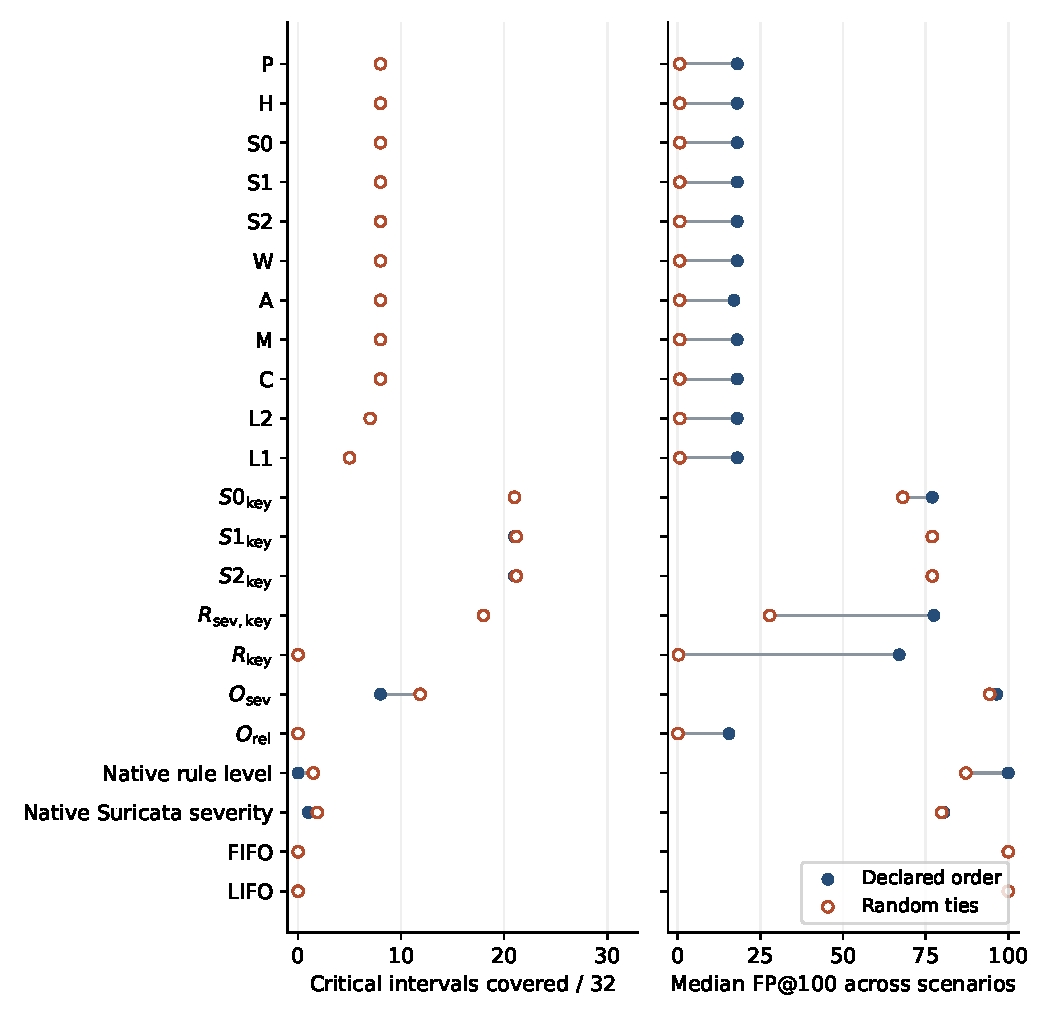
\includegraphics[width=\textwidth]{generated/figures/fig_static_tradeoff.pdf}
\caption{Declared and tie-averaged static outcomes for every ranker, with original selections fixed. Left: total interval coverage (mean over 100 permutations for random ties). Right: median FP@100 across scenarios (median of exact per-scenario expectations for random ties). Connected points show sensitivity to tie policy, not uncertainty intervals.}
\label{fig:static}
\end{figure}

\subsection{Ties decide class-level top-100 lists}
\label{subsec:ties}

Class-level scores take few distinct values, because $c$ and $h$ are constant within a mapped class. Each of the nine class-level formulas has 5--8 distinct finite score values per scenario; Online Resource~1, Section~S7 reports the counts for every formula and scenario. For every class-level formula score, at least \TieOrderShareMin\% of the top-100 positions in every scenario lay in tied score blocks (Table~\ref{tab:ties}). For P, the tied block crossing position 100 contained up to \TieBlockMax{} alerts. It supplied \TieCutoffMembersMinP--\TieCutoffMembersMaxP{} of the first 100 positions (median \TieCutoffMembersMedianP), so timestamp order determined which members entered the list. For the tuned A and M selections, the cutoff block supplied as few as \TieCutoffMembersMinClass{} positions. Class-level formula scores had identical coverage under all 100 within-block permutations, but false-positive counts varied. Under uniform ordering within tied blocks, the exact expected FP@100 of P has a median of \TieExpectedFPMedian{}, against \StaticClassFPMedian{} under the declared order. This contrast demonstrates sensitivity to secondary ordering. It does not show that chronology caused the advantage over severity-only: scores determine the prioritized blocks, while tie order selects members within them. The permutation diagnostic concerns a completed static queue. Section~\ref{sec:sensitivity} separately evaluates random priorities assigned causally on arrival; static permutations do not predict that replay outcome. S1\key{} had small cutoff blocks and nearly identical expected and declared FP; S0\key{} and \Rsev{} remained partly tie-dependent (median expected FP@100 of 68 and 28, against 77 and 77.5 declared).

\begin{tableorg}[t]
\centering
\caption{Essential tie diagnostics at $k=100$; all entries are medians over eight scenarios. Cutoff block: size of the tied block crossing rank 100. Selected from block: positions filled from that block. Expected FP: exact expectation under uniform within-block ordering. Online Resource~1, Section~S7 gives the full diagnostic, including tied shares and summed per-scenario coverage extrema; those extrema differ from the aggregate seed ranges in Table~\ref{tab:static}.}
\label{tab:ties}
\small
\begin{tabular}{lrrrr}
\toprule
Ranker & \shortstack{Cutoff\\block} & \shortstack{Selected\\from block} & \shortstack{Declared\\FP} & \shortstack{Expected\\FP} \\
\midrule
P & 213,201 & 96.5 & 18 & 0.6 \\
A & 213,201 & 66 & 17 & 0.6 \\
S0\textsubscript{key} & 5,548 & 22 & 77 & 68.1 \\
S1\textsubscript{key} & 24 & 7 & 77 & 77.0 \\
R\textsubscript{sev,key} & 214,931 & 60.5 & 77.5 & 27.8 \\
O\textsubscript{sev} & 102,064 & 96.5 & 96.5 & 94.4 \\
Native rule level & 679 & 96.5 & 100 & 87.2 \\
\bottomrule
\end{tabular}
\unskip
\end{tableorg}

\subsection{Why critical alerts are deferred}
\label{subsec:deferral}

The nine class-level formulas are P, H, W, A, C, M, S0, S1, and S2. Each placed \DeferredCritical{} of \NCriticalAlerts{} critical alerts (\DeferredShare\%) in the lower half of the queue, against \DeferredShareSeverity\% for severity alone. Under the fixed mapping thresholds and severity policy, \DeferredMappingRejected{} deferred critical alerts came from identifiers rejected by the phase mapping. The interval-precision threshold of 0.5 failed for identifiers raising \DeferredPrecisionRejected{} deferred alerts. The purity threshold of 0.7 failed for identifiers raising 8,856. These counts overlap and do not identify separate causal effects. Most deferred critical alerts occur in long exfiltration windows. Their rules also raise many interval-labelled negatives, leading to assignment to the low-reliability unknown class. For S0, the severity coefficient $1 + u\ln h$ was non-positive for \SZeroReversalShare\% of critical alerts, reversing severity order; the domain-constrained S1 and S2 removed the reversal but deferred the same alerts. Figure~\ref{fig:curves} shows how interval coverage and alert-level critical recall diverge. For identifier-level variants, interval coverage rises within the first hundred positions. For class-level scores, critical recall stays near zero until most of the queue has been read.

\begin{figure}[t]
\centering
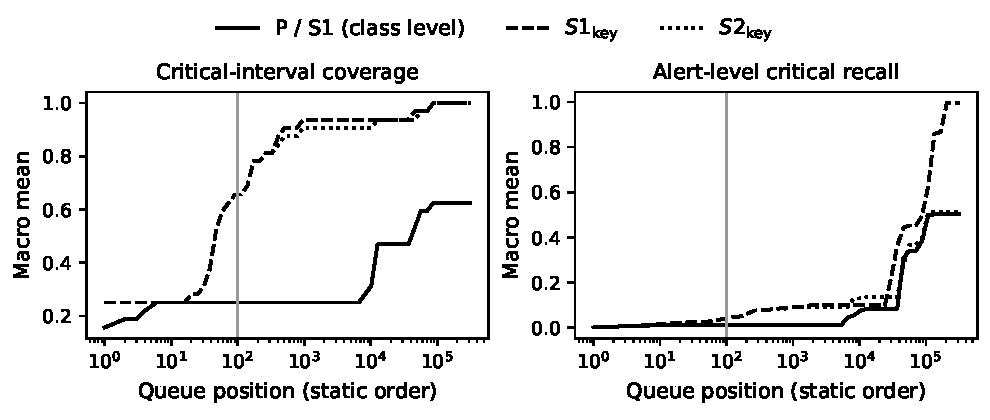
\includegraphics[width=\textwidth]{generated/figures/fig_rank_curves.pdf}
\caption{Critical-interval coverage (left) and alert-level critical recall (right) against queue position in the static order, macro-averaged over scenarios; evaluated at 200 log-spaced positions. The vertical line marks $k=100$.}
\label{fig:curves}
\end{figure}

\subsection{What drives coverage}
\label{subsec:drivers}

Table~\ref{tab:ablation} reruns the complete nested selection after changing one input. Coverage followed the granularity of reliability. With identifier-level precision, the class-level scores P and S1 covered 18 and 21 of 32 intervals, respectively, matching their identifier-level variants. Coarser or no reliability left coverage at 8 and raised median FP@100 to 96.5. Constant, historical-combined, precision-only, and purity-only uncertainty did not change coverage. Precision-only uncertainty lowered S1's median FP@100 to zero. Setting $u=0$ reduced the SGFN variants, including S1\key, to severity ordering and removed the identifier-level coverage gain. \Rsev, which uses no uncertainty, retained its gain. Asset context changed neither coverage nor, materially, false positives, and its factor was driven mostly by signature-name tokens rather than host or address information. Identifier-level methods are therefore not interchangeable: historical rule precision is a major driver of the observed coverage gain, while the formula and uncertainty interaction determine how that information is used. The primary mechanism is conditional on this policy; Section~\ref{sec:sensitivity} varies the mapping thresholds and reliability target.

\begin{tableorg}[t]
\centering
\caption{Input ablations with full nested reselection: covered intervals at $k=100$ (of 32) / median FP@100.}
\label{tab:ablation}
\small
\begin{tabular}{llcccc}
\toprule
Ablated input & Variant & P & S1 & S1\textsubscript{key} & R\textsubscript{sev,key} \\
\midrule
-- & detector-class (primary) & 8\,/\,18 & 8\,/\,18 & 21\,/\,77 & 18\,/\,77.5 \\
reliability & detector only & 8\,/\,96.5 & 8\,/\,96.5 & 21\,/\,77 & 18\,/\,77.5 \\
reliability & global class & 8\,/\,96.5 & 8\,/\,96.5 & 21\,/\,77 & 18\,/\,77.5 \\
reliability & native key & 18\,/\,77.5 & 21\,/\,77 & 21\,/\,77 & 18\,/\,77.5 \\
reliability & none & 8\,/\,96.5 & 8\,/\,96.5 & 21\,/\,77 & 18\,/\,77.5 \\
uncertainty & constant 0.5 & 8\,/\,18 & 8\,/\,18 & 21\,/\,77 & 18\,/\,77.5 \\
uncertainty & historical combined & 8\,/\,18 & 8\,/\,8 & 21\,/\,77 & 18\,/\,77.5 \\
uncertainty & precision only & 8\,/\,18 & 8\,/\,0 & 21\,/\,77 & 18\,/\,77.5 \\
uncertainty & purity only & 8\,/\,18 & 8\,/\,10 & 21\,/\,77 & 18\,/\,77.5 \\
uncertainty & zero & 8\,/\,18 & 8\,/\,96.5 & 8\,/\,96.5 & 18\,/\,77.5 \\
context & asset profile & 8\,/\,21 & 8\,/\,21 & 21\,/\,80.5 & 18\,/\,78 \\
\bottomrule
\end{tabular}
\unskip
\end{tableorg}

\begin{tableorg}[t]
\centering
\caption{Paired sign-flip tests with scenarios as units. Primary: prespecified family, Holm-adjusted. Exploratory: specified after results were seen, unadjusted. Differences are first minus second ranker; $+/-/0$ counts scenarios.}
\label{tab:tests}
\footnotesize
\begin{tabular}{lllrcrr}
\toprule
Family & Contrast & Outcome & Mean diff. & $+/-/0$ & Exact $p$ & Holm $p$ \\
\midrule
Primary & S1 $-$ A & coverage@100 & +0.000 & 0/0/8 & 1.000 & 1.000 \\
Primary & S1 $-$ A & FP@100 & +0.750 & 2/1/5 & 0.750 & 1.000 \\
Primary & S1 $-$ M & coverage@100 & +0.000 & 0/0/8 & 1.000 & 1.000 \\
Primary & S1 $-$ M & FP@100 & -0.250 & 0/1/7 & 1.000 & 1.000 \\
Primary & S1 $-$ P & coverage@100 & +0.000 & 0/0/8 & 1.000 & 1.000 \\
Primary & S1 $-$ P & FP@100 & +0.000 & 0/0/8 & 1.000 & 1.000 \\
\midrule
Exploratory & S1\textsubscript{key} $-$ S1 & covered intervals@100 & +1.625 & 7/0/1 & 0.016 & -- \\
Exploratory & S1\textsubscript{key} $-$ S1 & FP@100 & +44.875 & 7/1/0 & 0.016 & -- \\
Exploratory & S1\textsubscript{key} $-$ S1 & replay covered intervals & +2.125 & 8/0/0 & 0.008 & -- \\
Exploratory & S1\textsubscript{key} $-$ S1 & replay FP investigations & +216.000 & 8/0/0 & 0.008 & -- \\
Exploratory & S0\textsubscript{key} $-$ P & covered intervals@100 & +1.625 & 7/0/1 & 0.016 & -- \\
Exploratory & S0\textsubscript{key} $-$ P & FP@100 & +47.875 & 7/1/0 & 0.016 & -- \\
Exploratory & S0\textsubscript{key} $-$ P & replay covered intervals & +1.875 & 8/0/0 & 0.008 & -- \\
Exploratory & S0\textsubscript{key} $-$ P & replay FP investigations & +7.500 & 5/2/1 & 0.188 & -- \\
Exploratory & R\textsubscript{sev,key} $-$ P & covered intervals@100 & +1.250 & 6/0/2 & 0.031 & -- \\
Exploratory & R\textsubscript{sev,key} $-$ P & FP@100 & +46.750 & 7/1/0 & 0.016 & -- \\
Exploratory & R\textsubscript{sev,key} $-$ P & replay covered intervals & +1.500 & 7/0/1 & 0.016 & -- \\
Exploratory & R\textsubscript{sev,key} $-$ P & replay FP investigations & +2.875 & 3/2/3 & 0.688 & -- \\
\bottomrule
\end{tabular}
\unskip
\end{tableorg}

% =====================================================================================
\section{Chronological replay: interval coverage under persistent overload}
\label{sec:replay}

Static ranking assumes that all alerts of a completed scenario are available at once. The replay removes that assumption. Every tested rate was heavily overloaded. At 12 alerts per hour, each ranker started \ReplayInvestigations{} investigations across eight scenarios. Peak backlogs ranged from \PeakBacklogMin{} to \PeakBacklogMax{} alerts per scenario. Even at 60 alerts per hour, only \ReplaySixtyShare\% of all records could be investigated, with a scenario maximum of \ReplaySixtyShareMax\%. Because the analyst idles only when nothing is waiting, every ranker made the same number of investigations, so the rankers differ in which alerts they investigate rather than in how many.

\begin{tableorg}[t]
\centering
\caption{Replay at 12 alerts per hour, totals over eight scenarios. Each ranker starts \ReplayInvestigations{} investigations. Panel (a) separates coverage before the exclusive interval end from later coverage; panel (b) partitions starts into interval-negative, noncritical interval-positive, and critical records, whose counts sum to the total. Uninvestigated critical records and their share are measured at the scenario horizon.}
\label{tab:replay}
\small
\textbf{(a) Critical intervals}\par\medskip
\begin{tabular}{lrrrr}
\toprule
Ranker & Covered / 32 & Before end & At/after end & Uncovered \\
\midrule
P & 13 & 4 & 9 & 19 \\
S1 & 13 & 4 & 9 & 19 \\
S0\key & 28 & 6 & 22 & 4 \\
S1\key & 30 & 7 & 23 & 2 \\
S2\key & 29 & 6 & 23 & 3 \\
\Rsev & 25 & 6 & 19 & 7 \\
O\textsubscript{sev} & 8 & 1 & 7 & 24 \\
LIFO & 11 & 9 & 2 & 21 \\
FIFO & 0 & 0 & 0 & 32 \\
\bottomrule
\end{tabular}
\par\bigskip\textbf{(b) Alert records}\par\medskip
{\setlength{\tabcolsep}{4pt}
\begin{tabular}{lrrrrr}
\toprule
Ranker & \shortstack{Interval-\\negative} & \shortstack{Noncritical\\positive} & Critical & \shortstack{Uninvestigated\\critical} & \shortstack{Share\\(\%)} \\
\midrule
P & 9,285 & 2,170 & 53 & 9,151 & 99.4 \\
S1 & 9,285 & 2,170 & 53 & 9,151 & 99.4 \\
S0\key & 9,345 & 1,986 & 177 & 9,027 & 98.1 \\
S1\key & 11,013 & 237 & 258 & 8,946 & 97.2 \\
S2\key & 9,997 & 1,259 & 252 & 8,952 & 97.3 \\
\Rsev & 9,308 & 2,092 & 108 & 9,096 & 98.8 \\
O\textsubscript{sev} & 11,479 & 0 & 29 & 9,175 & 99.7 \\
LIFO & 11,284 & 91 & 133 & 9,071 & 98.6 \\
FIFO & 11,508 & 0 & 0 & 9,204 & 100.0 \\
\bottomrule
\end{tabular}
}
\unskip
\end{tableorg}

Table~\ref{tab:replay} and Figure~\ref{fig:replay} show the result. Identifier-level historical precision increased interval coverage: S1\key{} covered \ReplaySOneKeyCovered, S0\key{} \ReplaySZeroKeyCovered, and \Rsev{} \ReplayRSevKeyCovered{} of \NCriticalIntervals{} intervals. Every class-level formula score covered \ReplayClassCovered{} intervals; L1 and L2 covered 10 and 12, respectively, and FIFO covered \ReplayFIFOCovered. Replay produced a different false-positive pattern from static ranking. S0\key{} and \Rsev{} made \ReplaySZeroKeyFP{} and \ReplayRSevKeyFP{} false-positive investigations, close to the \ReplayClassFP{} of the class-level group, whereas S1\key{} made \ReplaySOneKeyFP. In every scenario S1\key{} covered more intervals than S1 and made more false-positive investigations (Table~\ref{tab:tests}; Figure~\ref{fig:paired}). S0\key{} and \Rsev{} covered more intervals than P, with small false-positive differences in both directions. The formula matters: additional coverage does not carry a fixed false-positive cost.

\begin{figure}[t]
\centering
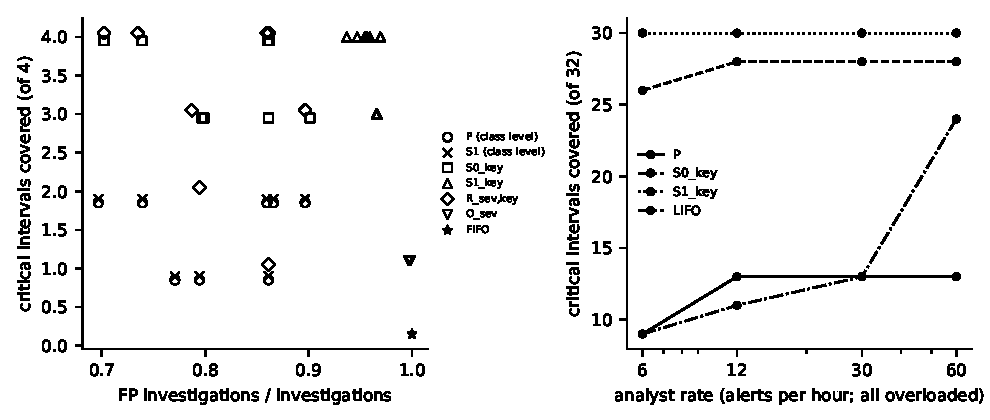
\includegraphics[width=\textwidth]{generated/figures/fig_replay.pdf}
\caption{Replay. Left: critical intervals covered against the share of investigations that were false positives at 12 alerts per hour, one point per scenario. Right: intervals covered at each tested rate; all rates were overloaded.}
\label{fig:replay}
\end{figure}

\paragraph{Coverage is not alert-level retrieval.} The ranker that covered \ReplaySOneKeyCovered{} of \NCriticalIntervals{} intervals investigated 258 of \NCriticalAlerts{} critical alerts and left \ReplaySOneKeyStarvedShare\% uninvestigated; the class-level group left \ReplayClassStarvedShare\% uninvestigated. Delay statistics among investigated alerts conceal this. For the rankers in Table~\ref{tab:delay}, every investigated critical alert entered service within 24 hours of arrival. Most covered intervals were first reached within an hour of their first alert. Rankers differed in the intervals and alerts still uninvestigated at the horizon. The horizon-truncated delay summary partly reflects those differences. Of the \ReplaySOneKeyCovered{} intervals covered by S1\key, only \RevisionBeforeSOneKey{} were first investigated before their end; \RevisionLateSOneKey{} were first investigated at or after it. For P, the corresponding counts were 4 and 9. Thus coverage within an hour of the first alert can coexist with investigation after a short attack interval has ended.

\begin{tableorg}[t]
\centering
\caption{Delay and coverage at 12 alerts per hour. The origin is the first alert inside each interval. Median delay is the median across scenarios of within-scenario medians among covered intervals. The median scenario mean lower-bound delay averages four interval delays within each scenario, substituting horizon minus origin for an uncovered interval, then reports the median of those eight means. Within 1 h counts covered intervals whose first qualifying investigation starts at most one hour after that origin. Horizons differ across scenarios; this is not a pooled restricted mean at a common follow-up time.}
\label{tab:delay}
\small
\begin{tabular}{lrrrr}
\toprule
Ranker & Covered (of 32) & \shortstack{Within\\1 h} & \shortstack{Covered median\\delay (h)} & \shortstack{Median scenario\\mean lower-bound\\delay (h)} \\
\midrule
S1\textsubscript{key} & 30 & 22 & 0.43 & 0.69 \\
S0\textsubscript{key} & 28 & 21 & 0.45 & 1.66 \\
R\textsubscript{sev,key} & 25 & 19 & 0.25 & 1.79 \\
P & 13 & 11 & 0.18 & 11.85 \\
O\textsubscript{sev} & 8 & 8 & 0.03 & 20.16 \\
FIFO & 0 & 0 & -- & 23.03 \\
\bottomrule
\end{tabular}

\unskip
\end{tableorg}

\paragraph{Limited sensitivity within the tested overload regime.} Coverage changed little across rates (Table~\ref{tab:rates}). From 6 to 60 alerts per hour, class-level formula scores covered 9--13 intervals. The identifier-level scores S0\key, S1\key, S2\key, and \Rsev{} covered 23--30, while LIFO rose from 9 to 24. Although aggregate arrivals exceeded capacity at every tested rate, the backlog could temporarily empty; utilization and idle time are reported in Online Resource~1. All tested rates were overloaded in aggregate, so these results describe sensitivity within that regime. They do not establish robustness when capacity approaches alert volume. At 12 alerts per hour, timestamp and hash order decided about 96\% of class-level and 76--84\% of identifier-level selections.

\begin{tableorg}[t]
\centering
\caption{Critical intervals covered (of 32) at each analyst rate; investigations are per ranker, totalled over the eight scenarios.}
\label{tab:rates}
\small
\begin{tabular}{lrrrrrrr}
\toprule
Rate (per h) & Investigations & P & S0\key & \Rsev & S1\key & S2\key & LIFO \\
\midrule
6 & 5,756 & 9 & 26 & 23 & 30 & 29 & 9 \\
12 & 11,508 & 13 & 28 & 25 & 30 & 29 & 11 \\
30 & 28,764 & 13 & 28 & 25 & 30 & 29 & 13 \\
60 & 56,941 & 13 & 28 & 25 & 30 & 29 & 24 \\
\bottomrule
\end{tabular}
\unskip
\end{tableorg}

\begin{figure}[!t]
\centering
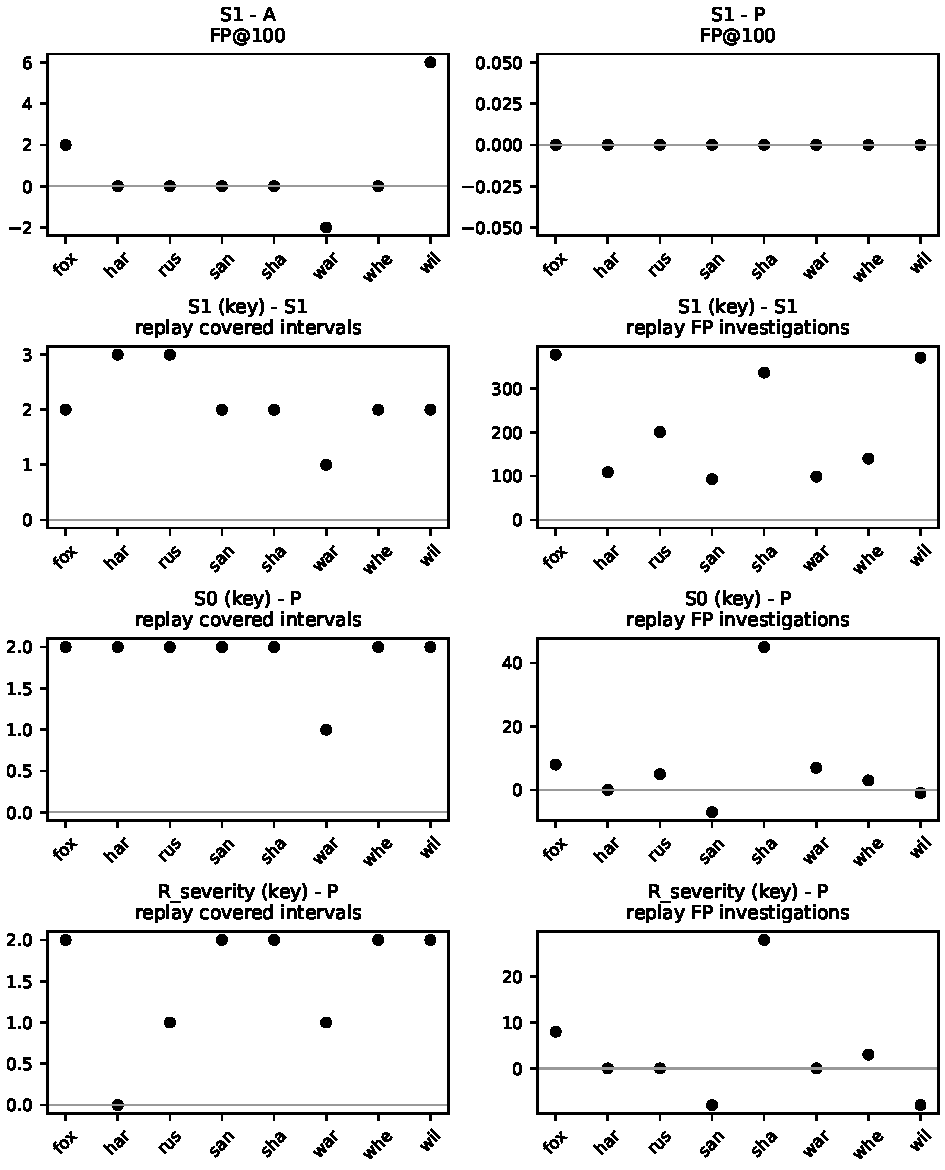
\includegraphics[width=0.90\textwidth]{generated/figures/fig_paired_effects.pdf}
\caption{Per-scenario paired differences. Top row: prespecified static FP@100 contrasts. Remaining panels: exploratory replay contrasts at 12 alerts per hour (unadjusted).}
\label{fig:paired}
\end{figure}
% =====================================================================================
\section{Generalization limits and temporal coverage versus confirmed detection}
\label{sec:generalization}

Leave-one-scenario-out evaluation contains little evidence about new identifiers: only \NUnseenAlerts{} held-out alerts came from identifiers absent from training, and none was critical. We therefore withheld five deterministic hash groups of identifiers from every fitting stage, including mapping, reliability, learned-model training, and inner validation. S1\key{} covered \HoldoutSOneKeyGroups{} of 32 intervals across groups 0--4, respectively (Online Resource~1, Table~S1). Four groups reduced coverage to 8--9, but group 1 retained 20; a universal failure-to-transfer claim is unwarranted.

The groups have unequal support (Table~\ref{tab:holdout-support}). Group 1 contains many alerts but only 63 critical records, whereas groups 0 and 4 contain 3,566 and 4,192 critical records. In the mixed top-100 queues, S1\key{} retrieves 2, 1, 8, 0, and 0 critical records from the withheld groups, covering 1/24, 1/18, 3/10, 0/26, and 0/32 intervals eligible for those groups. These subgroup fractions use only intervals containing a withheld-group alert; they are distinct from whole-queue coverage. The observed benefit is sensitive to which identifiers are excluded, and the experiment does not establish reliable transfer to new detector content.

In forward chaining, fitting uses only scenarios ending before the test scenario starts. Five test scenarios have at least two eligible training scenarios. In start-time order (UTC), these are russellmitchell (21 January 2022), shaw (25 January), wheeler (26 January), wilson (3 February), and harrison (4 February). Online Resource~1 lists their exact extents and fitting sets. Static S1\key{} covered \ForwardSOneKey{} and P \ForwardP{} of 20 critical intervals. The exploratory replay uses the same five test scenarios at 12 investigations per hour, regenerates the original nested selections, and verifies their saved static outcomes before replay (Table~\ref{tab:forward-replay}). This tests temporal isolation across scenarios within the same testbed, not deployment transfer.

\begin{tableorg}[t]
\centering
\caption{Identifier hold-out support and S1\key{} outcomes. Alerts and critical records are summed across scenarios. Eligible intervals contain at least one record from the withheld group. Subgroup covered counts only selected top-100 records from that group; whole coverage includes all identifiers.}
\label{tab:holdout-support}
\small
\begin{tabular}{lrrrrrr}
\toprule
Group & Keys & Alerts & \shortstack{Critical\\records} & \shortstack{Subgroup\\retrieved} & \shortstack{Subgroup\\covered/eligible} & \shortstack{Whole\\covered/32} \\
\midrule
0 & 15 & 496,247 & 3,566 & 2 & 1/24 & 9 \\
1 & 16 & 1,702,148 & 63 & 1 & 1/18 & 20 \\
2 & 20 & 21,326 & 49 & 8 & 3/10 & 8 \\
3 & 17 & 152,208 & 1,334 & 0 & 0/26 & 8 \\
4 & 25 & 283,892 & 4,192 & 0 & 0/32 & 8 \\
\bottomrule
\end{tabular}
\unskip
\end{tableorg}

\begin{tableorg}[t]
\centering
\caption{Replay on five forward-eligible scenarios (20 critical intervals); cells are LOSO / forward fitting. Both designs start 7,477 investigations per ranker at 12/h; forward fitting excludes later scenarios. Before end counts first starts before the exclusive interval end. The residual start category is noncritical interval-positive; Online Resource~1, Section~S9 gives the complete partition.}
\label{tab:forward-replay}
\small
\begin{tabular}{lrrrr}
\toprule
Ranker & Covered / 20 & Before end & Critical starts & \shortstack{Interval-negative\\starts} \\
\midrule
P & 7 / 6 & 2 / 1 & 27 / 20 & 5,994 / 6,821 \\
S1 & 7 / 6 & 2 / 1 & 27 / 20 & 5,994 / 6,821 \\
S0\key & 17 / 17 & 2 / 2 & 108 / 129 & 6,046 / 6,059 \\
S1\key & 19 / 19 & 3 / 3 & 164 / 164 & 7,152 / 7,147 \\
S2\key & 18 / 17 & 2 / 2 & 159 / 147 & 6,467 / 6,433 \\
\Rsev & 14 / 13 & 2 / 2 & 65 / 74 & 6,017 / 6,028 \\
O\textsubscript{sev} & 5 / 5 & 0 / 0 & 17 / 15 & 7,460 / 7,462 \\
LIFO & 6 / 6 & 5 / 5 & 95 / 95 & 7,325 / 7,325 \\
FIFO & 0 / 0 & 0 / 0 & 0 / 0 & 7,477 / 7,477 \\
\bottomrule
\end{tabular}
\unskip
\end{tableorg}

S1\key{} covered 19 of 20 intervals with either fitting design, but 16 were first investigated at or after their end. Forward fitting investigated 164 of 7,803 critical records and started 7,147 interval-negative investigations. P covered 6 intervals in forward replay versus 7 with LOSO fitting. Temporal isolation therefore preserves the large coverage--retrieval gap; the five scenarios do not establish general transfer.

All results rely on interval labels and an author-defined severity policy. An investigated alert inside a critical window may be unrelated to the attack step; an alert outside every window is not verified benign; and severity values encode assumptions rather than measured impact. The AIT scenarios are simulated, share infrastructure and attack tooling, and do not represent an operational SOC. No independent expert assessment of severity or of alert relevance was performed. The supplementary UWF-ZeekData24 analysis measures consistency between two author-defined severity tables and provides no independent severity validation.

% =====================================================================================
\section{Exploratory sensitivity to policy and investigation unit}
\label{sec:sensitivity}

\subsection{Mapping, shrinkage, severity, and reliability target}
The dated extension evaluates 23 configurations, including reproduction of the original setting, in 184 outer folds. The analysis retains all formula grids and operational references and repeats training-only mapping, cross-fitted reliability, and nested selection. It excludes the two learned families to focus on how explicit scoring formulas respond to input-policy changes. It does not assess the policy robustness of L1 or L2. Precision is varied over 0.3--0.7, purity over 0.5, 0.7, and 0.9, with four joint precision--purity corners. Support minima, shrinkage, severity, and criticality are varied separately (Online Resource~1, Section~S8). These settings are sensitivity cases, not a search for a new policy using test outcomes.

All nine class-level formulas still cover eight intervals in every configuration, although changing the criticality definition changes the denominator. Precision alone leaves S1\key{} at 21/32 intervals; raising purity to 0.9 reduces both S1\key{} and \Rsev{} to 8/32, including both joint corners with that purity. Shrinkage also matters: S1\key{} covers 23 intervals at $\lambda=0$ or 10 and 21 at 50 or 200, whereas \Rsev{} covers 11, 8, 18, and 21 respectively. A $+1$ shift to ranking severities with evaluation labels fixed reduces \Rsev{} to 8/32 while S1\key{} remains at 21/32. Thus the class-level coverage equality persists across these cases, but neither identifier-level gains nor their relative burden are independent of the author-defined policy.

The original reliability target is membership in any attack interval, whereas the primary endpoint concerns critical intervals. An ablation changes only the class/key reliability counts and their priors to critical membership, retaining the original phase mapping. P then defers 1,907 critical records beyond half the queue, compared with 9,047 originally, while S1 defers 9,092; both still cover eight intervals. S1\key{} covers 23 intervals but defers 8,966 records, versus 21 intervals and 1,802 deferred originally. Target alignment therefore changes deep-queue retrieval in a formula-dependent way and does not guarantee improvement. Precision and purity failures overlap; the original rejection counts alone cannot identify a single causal cutoff.

\subsection{Causal randomized ties}
For seven fixed original rankers, 100 seeded random priorities replace timestamp priority within equal-score backlog blocks. Priorities are deterministic functions of each alert's stable hash and seed, so they can be assigned on arrival without future information. Arrivals, scores, the 12/h service rate, and horizons are unchanged. Table~\ref{tab:review-random} summarizes totals across eight scenarios per seed. Seed means are first calculated within each scenario for exploratory paired tests; seeds do not enlarge the sample size.

S1\key{} averages 30.76 covered intervals and 282.34 critical starts; 96.93\% of critical records remain uninvestigated. P averages 13.98 covered intervals. The direction of their coverage--burden contrast persists (both scenario-paired exploratory $p=0.0078$), but severity-only coverage changes substantially, from 8 to a mean of 17.19. For severity-only ranking (O\textsubscript{sev}), timestamp-first ties yield coverage of 8, below every tested random-tie total both statically (10--14) and in replay (14--21). Comparisons against this reference therefore depend materially on tie policy; these observations do not establish a worst case over all possible tie orders. Random ties change comparisons with severity-only ranking, but the raw-record gap between coverage and retrieval remains. These results apply to this randomized tie policy, not to all causal schedulers.

\begin{tableorg}[htbp]
\centering\small
\caption{Raw-alert replay at 12/h: 11,508 starts per ranker and seed. FIFO ties uses timestamp-first ordering; remaining columns give random-tie means over 100 seed totals and coverage range (of 32). Before end counts first starts before the exclusive interval end. Online Resource~1, Section~S9 also reports noncritical interval-positive starts.}
\label{tab:review-random}
\resizebox{\textwidth}{!}{\begin{tabular}{lrrrrr}
\toprule
Ranker & FIFO ties & Random mean [range] & Before end & Critical starts & \shortstack{Interval-negative\\starts} \\
\midrule
P & 13 & 13.98 [13--14] & 6.83 & 64.6 & 9275.7 \\
S1 & 13 & 13.98 [13--14] & 6.83 & 64.6 & 9275.7 \\
S0\key & 28 & 28.63 [28--29] & 6.48 & 182.5 & 9335.7 \\
S1\key & 30 & 30.76 [30--31] & 7.57 & 282.3 & 10970.4 \\
S2\key & 29 & 29.63 [29--30] & 6.48 & 257.5 & 9985.8 \\
\Rsev & 25 & 25.63 [25--26] & 6.48 & 113.5 & 9298.8 \\
O\textsubscript{sev} & 8 & 17.19 [14--21] & 8.09 & 129.0 & 11250.7 \\
\bottomrule
\end{tabular}
}
\end{tableorg}

\subsection{Closed-group investigation}
Alerts are grouped by detector, native key, and host in windows anchored at the first member (60, 300, or 900 seconds). A group becomes selectable at window closure and takes the maximum member score; no member arrives at or after closure. The same analyst starts at most 12 group investigations per hour. The observation horizon remains the raw stream's first-to-last alert extent, without draining; groups closing later remain uninvestigated. Labels enter only after selection. Groups partition into critical (any critical member), noncritical-positive (a positive member but no critical member), and interval-negative (no positive member), including groups with mixed labels. An investigated group covers the union of its members' critical intervals at its service start, so future members cannot confer earlier coverage. Equal service per closed group is a workload assumption, not measured SOC productivity. Service time is held fixed across window lengths even though longer windows can place more records in each group, so the per-window comparison changes the workload represented by one investigation.

At 300 seconds, 2,655,821 records form 43,439 groups, of which 611 contain a critical record. S1\key{} covers 30 intervals, investigates 163/611 critical groups (26.68\%), and reaches 7 intervals before their end (Table~\ref{tab:review-grouped}). P covers 27 intervals, compared with 13 under raw-alert service. S0\key{} and \Rsev{} have identical displayed outcomes at 300 seconds, as verified in the saved per-scenario results; equality of these summaries does not establish identical selected groups. At 60/900 seconds, S1\key{} still covers 30 intervals and retrieves 14.49/37.05\% of critical groups. The investigation unit therefore changes both the between-ranker coverage gap and the retrieval denominator. The raw 97.2\% uninvestigated figure must not be read as a fraction of unresolved incidents. Grouping reduces that fraction under the stated model, while coverage and timely investigation remain distinct outcomes.

\begin{tableorg}[htbp]
\centering\small
\caption{Grouped replay with 300-second windows and 12 groups/h: 11,500 starts per ranker. Coverage is out of 32 intervals. Starts partition into interval-negative, noncritical-positive, and critical groups (Online Resource~1, Section~S9). Critical groups reports investigated / all critical groups, including those not released by the horizon. Critical members counts raw critical records contained in investigated groups; these are not separate investigations or confirmed attacks.}
\label{tab:review-grouped}
\resizebox{\textwidth}{!}{\begin{tabular}{lrrrrrr}
\toprule
Ranker & Covered & Before end & Critical groups & Retrieved (\%) & \shortstack{Interval-negative\\groups} & Critical members \\
\midrule
P & 27 & 5 & 113/611 & 18.49 & 11,007 & 259 \\
S1 & 27 & 5 & 113/611 & 18.49 & 11,071 & 259 \\
S0\key & 30 & 6 & 174/611 & 28.48 & 10,902 & 363 \\
S1\key & 30 & 7 & 163/611 & 26.68 & 11,250 & 260 \\
S2\key & 30 & 7 & 174/611 & 28.48 & 10,923 & 363 \\
\Rsev & 30 & 6 & 174/611 & 28.48 & 10,902 & 363 \\
O\textsubscript{sev} & 8 & 0 & 18/611 & 2.95 & 11,482 & 29 \\
\bottomrule
\end{tabular}
}
\end{tableorg}

\section{Discussion}
\label{sec:discussion}

\paragraph{Interpretation.} Under the primary input policy, historical rule precision is a major signal, whose effect depends on mapping purity, shrinkage, and the reliability target. Aggregation to mapped attack classes pushes rules that fire in benign and attack periods, including those raising most critical alerts, to the end of the queue; identifier-level precision lets some surface earlier. That benefit varies sharply across identifier hold-out groups and does not establish transfer to unseen content. Coarse scores also make tie-breaking part of the method: timestamp order selects most class-level top-100 members, and false-positive counts depend on the order within a large tied block. Evaluations should report a declared tie rule and tie-aware diagnostics~\citep{McSherryNajork2008TiedScores}.

\paragraph{Competing objectives and SGFN.} Interval coverage, false-positive burden, and critical-alert retrieval are different objectives. Under the primary input policy and raw-alert service, the highest-coverage ranker made the most false-positive investigations among identifier-level scores. It left almost all critical records uninvestigated. Simpler identifier-level scores achieved much of its coverage at lower burden. Randomized ties preserve that direction, while grouped service narrows the coverage gap and changes retrieval denominators. In these experiments, the ablations indicate that historical rule precision is a major contributor to the gains; they do not establish a general causal relationship. At class level, SGFN matched the simpler formulas on coverage; at identifier level, the simpler severity--precision product covered \StaticRSevKeyCovered{} intervals against \StaticSOneKeyCovered{} for S1\key{} statically, and \ReplayRSevKeyCovered{} against \ReplaySOneKeyCovered{} in replay. The lower-burden alternative depends on the input policy. In the static sensitivity analysis, \Rsev{} covers 8--21 intervals across the tested shrinkage values and falls to 8 after a $+1$ ranking-severity shift. S1\key{} retains 21--23 intervals under those changes. Raising mapping purity to 0.9 reduces both scores to 8/32. These static checks do not establish replay robustness under changed input policies.

\paragraph{Implications for alert management.} The results suggest four reporting practices for capacity-limited alert prioritization. First, the tie-breaking rule should be stated and reported as part of the method, because with coarse scores it selects most of the investigated set. Second, deep-queue deferral should be monitored. The rules raising most critical alerts were among those rejected by the mapping and frequently failed both precision and purity thresholds. Historical rule precision is therefore a useful diagnostic under this policy. This association has not been validated as a prospective prediction rule in an operational SOC. Third, interval coverage, timeliness, and retrieval should be reported with false-positive burden and an explicit investigation unit. A queue touching most intervals can leave many critical units uninvestigated; the fraction depends strongly on whether those units are raw records or groups. Fourth, a change in score should be assessed against identifiers withheld from fitting, since the gains observed here depend on identifier history and vary substantially across held-out groups. These practices support evaluation under limited capacity; the experiments do not establish that any tested score improves operational outcomes.

\paragraph{Scope of the comparison.} The original comparison covers scores computable from the frozen per-alert input block and makes no state-of-the-art claim. We also evaluated an exploratory training-only native-key adaptation of AIT's detector-rate score~\citep{Landauer2024AITADS,AITDetectorScoreImplementation}. It covered 0 of 32 intervals statically and 2 of 32 in replay. Because it uses duration-normalized normal-window inputs and changes the published grouping, it is an adaptation rather than a replication and lies outside the matched-input formula comparison. Its definition and full results are in Online Resource~1, Section~S4.

\paragraph{Threats to validity.} The evidence comes from eight scenarios of one simulated testbed family with overlapping training folds, author-defined severity policies, and interval-label proxies. The primary replay uses equal investigation times and raw alerts under aggregate overload. The exploratory extensions vary tie policy and use closed alert groups; equal per-group service time is also an assumption. Identifier hold-out and input-policy ablations remain static evaluations. Independent severity adjudication, operational incident labels, heterogeneous investigation costs, and a capacity regime near raw-alert volume remain untested. Exploratory contrasts and sensitivity analyses are distinguished from the original primary tests; their interpretation is conditional on this testbed. A planned expanded operational feature comparison and a redesigned cross-domain evaluation were deferred and not run.

% =====================================================================================
\section{Conclusion}
\label{sec:conclusion}

On the AIT Alert Dataset, historical rule granularity, score formula, tie ordering, and service constraints jointly affect which alerts are investigated. With class-level rule information, the choice of formula did not affect static critical-interval coverage: all nine class-level formula scores, SGFN included, covered the same number of intervals in every scenario. Identifier-level precision increases coverage under the declared policy, while formulas differ in false-positive burden and replay outcomes. Under the primary raw-alert replay, most intervals covered by the highest-coverage ranker are first investigated at or after their end, and almost all critical records remain uninvestigated. The sensitivity analyses distinguish that result from outcomes under alternative tie policies and investigation units. Identifier hold-out is heterogeneous, and forward replay tests only temporal isolation within the same testbed. The controlled comparison shows why interval coverage alone is insufficient to assess alert prioritization. Alert-prioritization evaluations should report coverage, timeliness, false-positive burden, and record-level retrieval together, state tie ordering, and report the support for held-out identifiers and scenarios.

\backmatter

\bmhead{Acknowledgements}

The author thanks the maintainers of the public datasets used in this study.

\section*{Statements and Declarations}

\begin{itemize}[leftmargin=*]
\item \textbf{Funding.} This research did not receive any specific grant from funding agencies in the public, commercial, or not-for-profit sectors.
\item \textbf{Competing interests.} The author declares that he has no known competing financial interests or personal relationships that could have appeared to influence the work reported in this paper.
\item \textbf{Ethics approval and consent to participate.} Not applicable. The study uses public datasets from simulated testbeds and involves no human participants.
\item \textbf{Consent for publication.} Not applicable.
\item \textbf{Data and code availability.} The AIT Alert Dataset (version 1) is available from Zenodo~\citep{AITAlertDataset2023} and UWF-ZeekData24 from the University of West Florida~\citep{Elam2025UWFZeekData24,UWFDatasetsPortal}, both under the Creative Commons Attribution 4.0 license. The archive contains analysis code, the frozen protocol, specifications and amendments, verification records, tests, outputs, derived tables, manuscript sources, and a reproduction guide. It also includes attributed derived AIT alert caches and the UWF-ZeekData24 subset used in the analysis. Raw AIT alert files are excluded. The reproducibility materials are available at \url{https://github.com/muratmoran/soc-alert-prioritization-reproducibility}. Release \texttt{v2026.10.30} provides the versioned archive, file checksums, and reproduction commands. No Zenodo DOI has been assigned. Original code is licensed under MIT, and original documentation and results under CC BY 4.0; third-party terms and manuscript rights remain separate.
\item \textbf{ORCID.} Murat Moran: 0000-0001-5557-4827.
\item \textbf{Author contributions.} Murat Moran: conceptualization, methodology, software, validation, formal analysis, investigation, data curation, visualization, writing---original draft, writing---review and editing, project administration.
\end{itemize}


\section*{Supplementary material}
Online Resource~1 (PDF): Detailed method specification, version comparison, supporting UWF analysis, rate-score adaptation, complete static outcomes, tie diagnostics, policy sensitivities, grouped and randomized replay, and the reproducibility inventory.

\bibliography{references}

\end{document}
